% !TEX root = main.tex
\section{System Design and Implementation}
% Section Overview
% Before we designed our system, we first implemented VQ and covq. We did this so we could expand on our code, but also so we could implement the independent decoders for comparing our system. We did implementation is C and Python, we also did some plotting in MATLAB. Mention that detailed design description is covered in design summary.
The new conditions of optimality presented in \eqref{} \eqref{} introduce some unique design problems, which we will discuss in this section.

In the subsequent sections we will detail the design challenges that were faced along the way and how they were addressed.

In the course of implementating this project, we began by writing a C program to perform simple \sysII\ Vector Quantization, and adapted it to an implementation of \sysIIN\ Channel-Optimized Vector Quantization by modifying the optimality conditions as was outlined in the Description section. We then wrote a C implementation of the \sysIJ\ system without a channel. To interface with images, we wrote a Python wrapper program. We also used GNU Octave, MathWorks MATLAB, and Python to produce data and create plots.

\subsection{Conditions of Optimality}
The new centroid condition we presented in equation \eqref{eq:cent_IJN} and the distortion measure of \eqref{eq:dist_IJN} can be expanded to reveal the relevant implementation issues. We begin by expanding the centroid condition of equation \eqref{eq:cent_IJN}: the optimal $X$ ($Y$ respectively) codebook $\{x_{k,l}\}$ ($\{y_{k,l}\}$ respectively) for an \sysIJN\ system with fixed encoder regions $R_i^X, R_j^Y$ is given by:
\begin{align}
    \label{eq:int_cent_IJN_x}
    x_{k,l}
    &= \frac{
        \sum_{i=1}^{N_X}\sum_{j=1}^{N_Y}
            P(k,l|i,j)\int_{R_i^X}xf_X(x)dx
    }{
        \sum_{i=1}^{N_X}\sum_{j=1}^{N_Y}
            P(k,l|i,j)P(X\in R_i^X, Y\in R_j^Y)
    }\\
    \label{eq:int_cent_IJN_y}
    y_{k,l}
    &= \frac{
        \sum_{i=1}^{N_X}\sum_{j=1}^{N_Y}
            P(k,l|i,j)\int_{R_j^Y}yf_Y(y)dy
    }{
        \sum_{i=1}^{N_X}\sum_{j=1}^{N_Y}
            P(k,l|i,j)P(X\in R_i^X, Y\in R_j^Y)
    }
\end{align}
where $f_X(\cdot)$, $f_Y(\cdot)$ are the marginal distributions of $X$ and $Y$ respectively.

Recall from the Lloyd algorithm of the previous section that we can approximate the expected value integrals, and the probability $P(X\in R_i^X, Y\in R_j^Y)$ with a training set drawn from the source distributions. Let $\mathcal T$ be a finite training set of ordered pairs drawn from the joint distribution for $X$ and $Y$. The integrals and the probability can be approximated as follows:

\begin{align}
    \int_{R_i^X}xf_X(x)dx&\approx
        \frac{1}{|\mathcal T|}\sum_{(x,y)\in \mathcal T}x\\
    \int_{R_i^Y}yf_Y(y)dy&\approx
        \frac{1}{|\mathcal T|}\sum_{(x,y)\in \mathcal T}y\\
    P(X\in R_i^X, Y\in R_j^Y)&\approx 
        \frac{\left|\{(x,y)\in \mathcal T\ |\ x\in R_i^X, y\in R_j^Y\}\right|
        }{
        |\mathcal T|
        }
\end{align}

Rewriting equations \eqref{eq:int_cent_IJN_x}, \eqref{eq:int_cent_IJN_y} in these terms, we get:
\begin{align}
    \label{eq:comp_cent_IJN_x}
    x_{k,l}
    &= \frac{
        \sum_{i=1}^{N_X}\sum_{j=1}^{N_Y}
            P(k,l|i,j)\sum_{(x,y)\in \mathcal T}x
    }{
        \sum_{i=1}^{N_X}\sum_{j=1}^{N_Y}
            P(k,l|i,j)
            \left|\{(x,y)\in \mathcal T\ |\ x\in R_i^X, y\in R_j^Y\}\right|
    }\\
    \label{eq:comp_cent_IJN_y}
    y_{k,l}
    &= \frac{
        \sum_{i=1}^{N_X}\sum_{j=1}^{N_Y}
            P(k,l|i,j)\sum_{(x,y)\in \mathcal T}y
    }{
        \sum_{i=1}^{N_X}\sum_{j=1}^{N_Y}
            P(k,l|i,j)
            \left|\{(x,y)\in \mathcal T\ |\ x\in R_i^X, y\in R_j^Y\}\right|
    }
\end{align}

These terms are simple to compute, and as in the more simple \sysJJN\ case, depend only on the encoding regions $R_i^X, R_J^Y$, the channel probability $P(k,l|i,j)$, and the training set $\mathcal T$.

Similarly, we write out the nearest neighbour conditions; the idea is the same as in COVQ. The optimal encoding partitions $R_i^X$ for $X$ (respectively $R_j^Y$ for $Y$) given fixed partitions in $Y$ (respecitvley $X$), and fixed codebook $\mathcal C=\{(x_{k,l},y_{k,l})\}$ are given by:
\begin{align}
    \label{eq:NN_part_X}
    R_i^X &=
        \{x\ |\ d(x, i) \le d(x, h), \forall h\in \{1,...,N_X\}\}\\
    \label{eq:NN_part_Y}
    R_j^Y &=
        \{y\ |\ d(y, j) \le d(y, h), \forall h\in \{1,...,N_Y\}\}
\end{align}
where, expanding for $d(x,i), d(y,j)$ from equations \eqref{eq:dist_IJN_x}, \eqref{eq:dist_IJN_y} gives us:
\begin{align}
    \label{eq:int_dist_x}
    d(x,i)=&E[Y^2 | X = x] +\\
    &\sum_{j=1}^{N_Y} \sum_{k=1}^{N_X} \sum_{l=1}^{N_Y} ( {(x-x_{(k,l)})}^2 -
    2y_{(k,l)}E[Y|X=x,Y\in R_j^Y] + y_{(k,l)}^2 )P(Y\in R_j^Y|X=x)
    P(k,l|i,j)\nonumber\\
    \label{eq:int_dist_y}
        d(y,j)=&E[X^2 | Y = y] +\\
    &\sum_{i=1}^{N_X} \sum_{k=1}^{N_X} \sum_{l=1}^{N_Y} ( {(y-y_{(k,l)})}^2 -
    2x_{(k,l)}E[X|Y=y,X\in R_i^X] + x_{(k,l)}^2 )P(X\in R_i^X|Y=y)
    P(k,l|i,j)\nonumber
\end{align}

Here, we note how the nearest neighbour condition for $X$ depends on the $Y$ encoding regions $\{R_j^Y\}$, and vice versa. It is therefore necessary to adapt the Lloyd-Max iteration into three stages: the optimization of the $R_i^X$, the optimization of the $R_j^Y$, and the optimization of the codebook $\mathcal C=\{x_{k,l},y_{k,l}\}$. It is not clear what order of rotation between the three conditions is best, so in our system, we have chosen to give each one a single turn per Lloyd iteration.

There is another more pressing matter with regards to computing equations \eqref{eq:int_dist_x} and \eqref{eq:int_dist_y}. Focusing on $d(x,i)$, since $d(y, j)$ is analogous, the terms that present a new problem are:
\begin{align}
    \label{eq:problem_1}
    E[Y^2 | X = x]&=\int_{-\infty}^{\infty}y^2f_{Y|X}(y|x)\\
    \label{eq:problem_2}
    E[Y|X=x,Y\in R_j^Y]&=\frac{1}{P(Y\in R_j^Y)}\int_{R_j^Y}yf_{Y|X}(y|x)dy\\
    \label{eq:problem_3}
    P(Y\in R_j^Y|X=x)&=\int_{R_j^Y}f_{Y|X}(y|x)dy
\end{align}

Each one of these terms will need to be computed for a given $x$ in the support of $X$. Specifically, we need to approximate the conditional density function $f_{Y|X}(y|X=x)$ for all $x$ in the support of $X$. Otherwise, there will be some $x$ in the support of $X$ which we will not be able to encode via our nearest neighbour condition \eqref{eq:NN_part_X}. In order to ensure that this problem does not occur, we can approximate the conditional density with a discretized density function, in essence a probability mass function (pmf) of a discretized pair of random variables. To do so, we uniformly quantize the sources into `bins' that cover the supports of $X$ and $Y$.

Define
$q_X(x):\mathbb{R} \rightarrow \{\bar x_1,\ldots,\bar x_{L_X}\}$
and
$q_Y(y):\mathbb{R} \rightarrow \{\bar y_1,\ldots,\bar y_{L_Y}\}$
to be the $L_X$- and $L_Y$-level uniform quantizers for the sources $X$ and $Y$ respectively, where the $\bar x_i-\bar x_{i-1}$ is constant for all $i\in \{2,\ldots,L_X\}$, and $\bar y_i-\bar y_{i-1}$ constant for all $i\in \{2,\ldots,L_Y\}$. Call these constants respectively $\Delta_X, \Delta_Y$.
\begin{align}
    q_X(x) = \bar x_i \in \{\bar x_1,\ldots,\bar x_{L_X}\} &\iff x \in  \left[\bar x_{i}-\frac{\Delta_X}{2},\ \bar x_i+\frac{\Delta_X}{2}\right)\\
    q_Y(y) = \bar y_i \in \{\bar y_1,\ldots,\bar y_{L_Y}\} &\iff y \in  \left[\bar y_{i}-\frac{\Delta_Y}{2},\ \bar y_i+\frac{\Delta_Y}{2}\right)
\end{align}
with the convention that $\bar x_{0}=\bar y_{0}=-\infty$, and $\bar x_{L_X+1}=\bar y_{L_Y+1}=+\infty$.

Call the uniformly quantized random variables $\bar X, \bar Y$. We can then approximate the conditional densities $f_{Y|X}, f_{X|Y}$ with the densities of the $\bar X, \bar Y$ as follows. Define $f_{\bar Y|\bar X},f_{\bar X|\bar Y}$ to be the conditional densities of the pair $\bar X, \bar Y$:
\begin{align}
    \label{eq:quant_pdf_x}
    f_{\bar Y|\bar X}(y|x) =\frac{f_{\bar X,\bar Y}(x,y)}{f_{\bar X}(x)}=
        \frac{
            \int_{q_X(x)-\Delta_X}^{q_X(x)+\Delta_X}
            \int_{q_Y(y)-\Delta_Y}^{q_Y(y)+\Delta_Y}
                f_{X,Y}(x',y')dy'dx'
        }{
            \int_{q_X(x)-\Delta_X}^{q_X(x)+\Delta_X}f_X(x')dx'
        }\approx f_{Y|X}(y|x)\\
    \label{eq:quant_pdf_y}
    f_{\bar X|\bar Y}(x|y) =\frac{f_{\bar X,\bar Y}(x,y)}{f_{\bar Y}(y)}=
        \frac{
            \int_{q_X(x)-\Delta_X}^{q_X(x)+\Delta_X}
            \int_{q_Y(y)-\Delta_Y}^{q_Y(y)+\Delta_Y}
                f(x',y')dy'dx'
        }{
            \int_{q_Y(y)-\Delta_Y}^{q_Y(y)+\Delta_Y}f_Y(y')dy'
        }\approx f_{Y|X}(y|x)
\end{align}
Notice that \eqref{eq:quant_pdf_x} (\eqref{eq:quant_pdf_y} resp.) is well defined and is a valid density assuming that $x$ ($y$ resp.) is in the support of $\bar X$ ($\bar Y$ resp.).

We can now approximate these two equations with a uniformly quantized training set from the sources $X, Y$. We call this uniformly quantized training set $\mathcal{\bar T}$:
\begin{align}
    \mathcal{\bar T}=\{(q_X(x'),q_Y(y'))\ |\ (x',y')\in \mathcal T\}
\end{align}
Define $p(x,y)$ as the joint \emph{empirical} distribution of $\mathcal{\bar T}$:
\begin{align}
    p(x,y) = \frac{
        |\{(x',y')\in \mathcal{\bar T}\ |\ (x',y')=(x,y)\}|
        }{
        |\mathcal{\bar T}|
        }
\end{align}
Similarly, define $p_X, p_Y, p_{Y|X},p_{X|Y}$ to be respectively, the empirical marginal distribution of $\bar X$, empirical marginal distribution of $\bar Y$, and empirical conditional distributions from the training set $\mathcal{\bar T}$:
\begin{align}
    p_X(x) &= \frac{
        |\{(x',y')\in\mathcal{\bar T}\ |\ x'=x\}|
    }{
        |\mathcal{\bar T}|
    }\\
    p_Y(y) &= \frac{
        |\{(x',y')\in\mathcal{\bar T}\ |\ y'=y\}|
    }{
        |\mathcal{\bar T}|
    }\\
    \label{eq:cond_pmf_y}
    p_{Y|X}(y|x) = \frac{p(x,y)}{p_X(x)}
    &= \frac{
            |\{(x',y')\in \mathcal T\ |\ q_X(x')=q_X(x),\ q_Y(y')=q_Y(y)\}|
        }{
            |\{(x',y')\in \mathcal T\ |\ q_X(x')=q_X(x)\}|
        }\approx f_{\bar Y|\bar X}(y|x)\\\
    p_{X|Y}(x|y) = \frac{p(x,y)}{p_Y(y)}
    &=  \frac{
            |\{(x',y')\in \mathcal T\ |\ q_X(x')=q_X(x),\ q_Y(y')=q_Y(y)\}|
        }{
            |\{(x',y')\in \mathcal T\ |\ q_Y(y')=q_Y(y)\}|
        }\approx f_{\bar X|\bar Y}(x|y)
\end{align}

We now rewrite our approximated versions of equations \eqref{eq:problem_1}, \eqref{eq:problem_2}, \eqref{eq:problem_3} (and their counterparts in $Y$). Define $T(x),T(y),M(x,j),M(y,i),S(x,j),S(y,i)$:
\begin{align*}
    T(x) &= \sum_{(x',y')\in \mathcal{\bar T}|x'=x}(y')^2p_{Y|X}(y'|x')\\
    T(y) &= \sum_{(x',y')\in \mathcal{\bar T}|y'=y}(x')^2p_{X|Y}(x'|y')\\
    M(x,j) &= \frac{|\mathcal{\bar T}|\sum_{(x',y')\in \mathcal{\bar T}|y'\in R_j^Y}y'p_{Y|X}(y|x)}{|\{(x',y')\in \mathcal{\bar T}\ |\ y'\in R_j^Y\}|}\\
    M(y,i) &= \frac{|\mathcal{\bar T}|\sum_{(x',y')\in \mathcal{\bar T}|x'\in R_i^X}x'p_{X|Y}(x|y)}{|\{(x',y')\in \mathcal{\bar T}\ |\ x'\in R_i^X\}|}\\
    S(x,j) &= \sum_{(x',y')\in \mathcal{\bar T}|y'\in R_j^Y}p_{Y|X}(y|x)\\
    S(y,i) &= \sum_{(x',y')\in \mathcal{\bar T}|x'\in R_i^X}p_{X|Y}(x|y)
\end{align*}

We now have all the means to rewrite out approximated distortion measures in computable terms via the uniformly quantized training set $\mathcal{\bar T}$. For simplicity of design, we in fact attach the uniform quantizer to the beginning of our system. That is, we essentially transform the sources such that they have (finite) state spaces of size $L_X, L_Y$ before performing the \sysIJN\ , (\sysIJ) training, or simulation (Refer to Modified block diagram). It is important to note that this design simplification affects the values of the distortions of equations \eqref{eq:int_dist_x} and \eqref{eq:int_dist_y} as well as the centroids computed via equations \eqref{eq:comp_cent_IJN_x}, \eqref{eq:comp_cent_IJN_y}; the distance with respect to which we are now optimizing is the expected distance from reconstruction to uniformly quantized source. In the following distortion measures, this is represented by the subscripts $\bar X,\bar Y$. We have:
\begin{align}
    \label{eq:NN_X}
    d_{\bar X}(x,i) =
            T(x) + 
            \sum_{j=1}^{N_Y} \sum_{k=1}^{N_X} \sum_{l=1}^{N_Y}
            \left(\left({(x-x_{k,l})}^2 +
            y_{k,l}^2\right)M(x,j) -2y_{k,l}S(x,j)\right)P(k,l|i,j)\\
    \label{eq:NN_Y}
    d_{\bar Y}(y,j) =
            T(y) + 
            \sum_{i=1}^{N_X} \sum_{k=1}^{N_X} \sum_{l=1}^{N_Y}
            \left(\left({(y-y_{k,l})}^2 +
            x_{k,l}^2\right)M(y,i) -2x_{k,l}S(y,j)\right)P(k,l|i,j)
\end{align}

\eqref{eq:NN_X} and \eqref{eq:NN_Y} are now easily computable for given pair $(x, i)$ or $(y, j)$, so the nearest neighbour optimization steps reduce to performing a search over codebook indicies $i$ ($j$ respectively) for the minimizing argument to $d_{\bar X}(x,i)$ ($d_{\bar Y}(y,j)$ respectively) for a given source pair $(x,y)\in \mathcal{\bar T}$.

We also note that, besides aiding notation, the terms $M(x,j),S(x,j),T(x)$, and their counterparts $M(y,i),S(y,i),T(y)$ can be computed initially, independent of $x, y$ respectively, reducing the computational complexity of the nearest neighbour search.

As mentioned above, applying the uniform quantizer at the beginning of our system also modifies the calculation of the centroids. We now write out the centroid condition in terms of the uniformly quantized training set $\mathcal{\bar T}$. We reiterate that the encoding partitions $\{R_i^X\}_{i=1}^{N_X}, \{R_j^Y\}_{j=1}^{N_Y}$ are held constant in the application of this condition.

Let $M_{(i,j)}$ be the number of training vectors that belong to $R_i\times S_j$:
\begin{align}
    M_{(i,j)} &=
    \sum_{\substack{(x,y)\in \mathcal{\bar T}:\\x\in R_i^X,y\in R_j^Y}}p(x,y)
\end{align}
and let $S_{(i,j)}^X$, $S_{(i,j)}^Y$ be given by:
\begin{align}
    S^X_{(i,j)} &=
    \sum_{\substack{(x,y)\in \mathcal{\bar T}:\\x\in R_i^X,y\in R_j^Y}}x p(x,y)\\
    S^Y_{(i,j)} &=
    \sum_{\substack{(x,y)\in \mathcal{\bar T}:\\x\in R_i^X,y\in R_j^Y}}y p(x,y)
\end{align}

With the above notation, the reconstructions that minimize distortion from $\mathcal{\bar T}$ to reconstruction are:
\begin{align}
    \label{eq:C_X}
    x_{(k,l)} = 
        \frac{\sum_{i=1}^{N_X} \sum_{j=1}^{N_Y}
        S_{(i,j)}^X P(k,l|i,j)}
        {\sum_{i=1}^{N_X} \sum_{j=1}^{N_Y}
        M_{(i,j)} P(k,l|i,j)}\\
    \label{eq:C_Y}
    y_{(k,l)} = 
        \frac{\sum_{i=1}^{N_X} \sum_{j=1}^{N_Y}
        S_{(i,j)}^Y P(k,l|i,j)}
        {\sum_{i=1}^{N_X} \sum_{j=1}^{N_Y}
        M_{(i,j)} P(k,l|i,j)}
\end{align}
Equations \eqref{eq:C_X}, \eqref{eq:C_Y} are again easily computable when our encoders are fixed.

Adding the uniform quantizer to the system presents us with new parameters. These are namely the choice of $\{\bar x_1, \bar y_1, \bar x_{L_X}, \bar y_{L_Y}, L_X, L_Y\}$ from the definitions of $q_X,q_Y$. Together, these parameters control the granularity of quantization, and position of the quantizer. For our simulations, we chose to (a) center the quantizer about the sample mean of $\mathcal T$, (b) pick $\{x_1, y_1, x_{L_X}, y_{L_Y}\}$ such that all of $\mathcal T$ lies within the square defined by the four terms. With these decisions, the only remaining parameter is simply how fine the quantizer ought to be.

For a given training set $\mathcal T$, we want fine enough quantization so to not distort the equations \eqref{eq:NN_X} and \eqref{eq:NN_Y} from the true source-to-reconstruction distortions, but coarse enough so that the conditional probabilities are well-defined for most bins. It is clearly the case that with a larger training set $\mathcal T$, we can use finer quantizations while maintaining well-defined bins. For our purposes, we iterate through values of $L_X, L_Y$, choosing the result with lowest average distortion.

It is also important to note that the computational complexity depends primarily on the numbers $L_X, L_Y$, not the size of $\mathcal T$, as was the case in the I$\rightarrow$I system.

As was mentioned in this section, the fact that there are now three necessary conditions for optimality necessitates a decision in the order of their application in the quantizer training stage. We chose to give equal opportunities to each condition, beginning with one of the encoders. There are clearly other possible rotation schemes that might provide an advantage. These are not explored in this paper.

To summarize this section, we present the procedure which we dub the `Channel Optimized Stage' of our algorithm. Assuming we are given a codebook of size $N_X N_Y$, and the encoding mappings $\mathcal E_X, \mathcal E_Y$, we apply our modified Lloyd-Max algorithm to obtain a better set of encoding mappings and codebook.

\begin{enumerate}
    \item Store the previous distortion value, $D_{avg}$.
    \item Quantize the training set $\mathcal T$ to $\mathcal{\bar T}$:
    \begin{align}
        \mathcal{\bar T}=\{(q_X(x),q_Y(y))\ |\ (x,y)\in \mathcal T\}
    \end{align}
    \item Update the $X$ encoder; for each $\bar x_m\in \{\bar x_1,\ldots,\bar x_{L_X}\}$, let
    \begin{align}
        \mathcal E_{\bar X}(\bar x_m)=\argmin_{i\in\{1,\ldots,N_X\}}d_{\bar X}(\bar x_m,i)
    \end{align}
    \item Update the $Y$ encoder; for each $y_n\in \{\bar y_1,\ldots,\bar y_{L_Y}\}$, let
    \begin{align}
        \mathcal E_{\bar Y}(\bar y_n)=\argmin_{j\in\{1,\ldots,N_Y\}}d_{\bar Y}(\bar y_n,j)
    \end{align}
    \item Update the codebook; for each $k\in\{1,\ldots,N_X\}$, $l\in\{1,\ldots,N_Y\}$ let
    \begin{align}
        x_{(k,l)} = 
            \frac{\sum_{i=1}^{N_X} \sum_{j=1}^{N_Y}
            S_{(i,j)}^X P(k,l|i,j)}
            {\sum_{i=1}^{N_X} \sum_{j=1}^{N_Y}
            M_{(i,j)} P(k,l|i,j)}\\
        y_{(k,l)} = 
            \frac{\sum_{i=1}^{N_X} \sum_{j=1}^{N_Y}
            S_{(i,j)}^Y P(k,l|i,j)}
            {\sum_{i=1}^{N_X} \sum_{j=1}^{N_Y}
            M_{(i,j)} P(k,l|i,j)}
    \end{align}
    \item Repeat until the average distortion changes less than a desired positive threshold, $\delta$; repeat if
    \begin{align}
        \frac
        {(D_{avg} - D^*_{avg})}
        {D_{avg}}
        > \delta
    \end{align}
    \\
    where $D_{avg}$ is the distortion of the previous iteration, and the new distortion $D^*_{avg}$ is given by
    \begin{align}
        D^*_{avg}=\sum_{m=1}^{L_X}\sum_{n=1}^{L_Y}p(\bar x_m,\bar y_n)\left(d_{\bar X}(\bar x_m,\mathcal E_X(\bar x_m))+d_{\bar Y}(\bar y_n,\mathcal E_Y(\bar y_n))\right)
    \end{align}
\end{enumerate}

% Note this decision is somewhat arbitrary, the effects of other choices of order haven't been studied

% Design Problems: 
% Need conditional distributions for nearest neighbour condition -> Use Uniform Quantizer.
% Need to consider bin size. Bins too big and uniform quantizer adds distortion. Make bins too small and you can't approximate conditional distribution very well. Need a lot of training points for good approximation. 

% Another thing to note: complexity depends on total number of bins rather than number of training points.

% Present equations for conditions of optimality for training set/quantizer.

\subsection{Codebook Initialization}
% Describe problem
% Considered different methods of codebook initialization.

Since each nearest neighbour condition depends on the encoding regions of the other source and the codebook pairs $(x_{(k,l)},y_{(k,l)})$ of the decoder, and the joint centroid conditions depend on the encoding regions for both sources, it is necessary to appropriately find either (a) initial encoding regions $\{R_i\}, \{S_j\}$ for the encoders or (b) initial encoding regions for one of the sources and initial reconstruction points $\{(x_{(k,l)}, y_{(k,l)})\}$ for the decoder. We decided to do both, exploring a couple strategies.

% How did this work? we initialize reconstruction points, but then we still need to initialize one of the encoders..
% One method we tried was to initialize the reconstruction points $\{(x_{(k,l)}, y_{(k,l)})\}$ to the first $N_X\cdot N_Y$ training pairs in $\mathcal T$. This would ensure that the initial codebook would have the same distribution as $\mathcal T$ assuming that samples of $\mathcal T$ are independent and identically distributed. However, we found that 

To make finding initial encoding regions simpler, we took a heuristic approach to firstly initialize a codebook of the desired size, $\mathcal C=\{(x_{(k,l)}, y_{(k,l)})\}$, $k=1\ldots N_X$, $l=1\ldots N_Y$, then apply suitable conditions to find initial encoding regions for \emph{both} sources, and finally begin the main iteration.

To find our initial codebook, our inspiration came from the Linde-Buzo-Gray (LBG) Splitting Algorithm. Recall that the LBG algorithm initializes the codebook to a single codevector, usually placed at the `center of mass' of the source distribution with respect to a distortion measure. We proceed in the same way, initially letting $N_X=N_Y=1$, with initial codebook pair $(x_{1,1},y_{1,1})$ given by:
\begin{align}
    x_{1,1} = \sum_{m=1}^{L_X}\sum_{n=1}^{L_Y}\bar x_m p(\bar x_m, \bar y_n)\\
    y_{1,1} = \sum_{m=1}^{L_X}\sum_{n=1}^{L_Y}\bar y_n p(\bar x_m, \bar y_n)
\end{align}
which are respectively the expected values of the uniformly quantized training set $\mathcal T$ for $X$ and $Y$. Trivially, our encoders at this point are given by:
\begin{align}
    \mathcal E_X(x) = 1\\
    \mathcal E_Y(y) = 1
\end{align}

We then define the average distortion from this choice of codebook as the expected value of the sum of the squared error distortion between the quantized training vectors in $\mathcal T$ and the codebook:
\begin{align}
    D^*_{avg}=\sum_{m=1}^{L_X}\sum_{n=1}^{L_Y}p(\bar x_m,\bar y_n)\left((\bar x_m-x_{1,1})^2+(\bar y_n-y_{1,1})^2\right)\\
\end{align}

We then split in the $X$ and apply a modified Lloyd iteration described as follows.
\begin{enumerate}
    
    \item \label{init_split} Split in $X$: let $N_X=2N_X$.
    \item \label{init_start} Remember previous distortion; let $D_{avg}=D^*_{avg}$
    \item Update the $X$ encoder; for each $\bar x_m\in\{\bar x_1,\ldots,\bar x_{L_X}\}$ let
    \begin{align}
        \mathcal E_X(\bar x_m) = \argmin_{i \in \{1,\dots,N_X\}}d_{\bar X}(\bar x_m,i)
    \end{align}
    where $d_{\bar X}(\bar x_m,i)$ is given as in \eqref{eq:NN_X}, however with zero probability of channel error reduces to:
    \begin{align}
        \label{eq:no_channel_NN_X}
        d_{\bar X}(\bar x_m,i) =
            T(\bar x_m) + 
            \sum_{j=1}^{N_Y}
            \left(\left({(\bar x_m-x_{i,j})}^2 +
            y_{i,j}^2\right)M(\bar x_m, j) -2y_{i,j}S(\bar x_m, j)\right)
    \end{align}
    \item Update the $X$ codebook values; for each $k\in \{1,\ldots,N_X\}$, $l\in\{1,\ldots,N_Y\}$, let
    \begin{align}
        x_{k,l} = 
            \frac{\sum_{(\bar x_m,\bar y_n)\in R_i^X\times R_j^Y}\bar x_m p(\bar x_m,\bar y_n)}
            {\sum_{(\bar x_m,\bar y_n)\in R_i^X\times R_j^Y}p(\bar x_m,\bar y_n)}
    \end{align}
    Notice that this is the expected value of the partition $(i,j)$.
    \item Update the $Y$ encoder; for each $\bar y_n\in \{\bar y_1,\ldots,\bar y_{L_Y}\}$, let
    \begin{align}
        \mathcal E_Y(\bar y_n) = \argmin_{j\in\{1,\ldots,N_Y\}}d_{\bar Y}(\bar y_n,j)
    \end{align}
    where $d_{\bar Y}(\bar y_n,j)$ is given as in \eqref{eq:NN_Y}, however with zero probability of channel error:
    \begin{align}
        \label{eq:no_channel_NN_Y}
        d_{\bar Y}(\bar y_n,j) =
            T(\bar y_n) + 
            \sum_{i=1}^{N_X}
            \left(\left({(\bar y_n-x_{i,j})}^2 +
            y_{i,j}^2\right)M(\bar y_n, i) -2y_{i,j}S(\bar y_n, i)\right)
    \end{align}
    \item Update the $Y$ codebook values; for each $k\in \{1,\ldots,N_X\}$, $l\in\{1,\ldots,N_Y\}$, let
    \begin{align}
        y_{k,l} = 
            \frac{\sum_{(\bar x_m,\bar y_n)\in R_i^X\times R_j^Y}\bar y_n p(\bar x_m,\bar y_n)}
            {\sum_{(\bar x_m,\bar y_n)\in R_i^X\times R_j^Y}p(\bar x_m,\bar y_n)}
    \end{align}
    \item Define the average distortion. let
    \begin{align}
        D_{avg}^* = \sum_{n=1}^{L_Y}d_{\bar Y}(\bar y_n, \mathcal E_Y(\bar y_n))\left(\sum_{m=1}^{L_X}p(\bar x_m,\bar y_n)\right)
    \end{align}
    \item
    \begin{enumerate}
        \item
        If
        $\frac
        {(D_{avg} - D^*_{avg})}
        {D_{avg}}
        > \delta$
        then return to step \ref{init_start},
        \item
        otherwise if $N_X$ is less than desired, go to next split (step \ref{init_split}),
        \item
        otherwise finish.
    \end{enumerate}
\end{enumerate}

After convergence of the algorithm for our final value of $N_X$, we then apply the symmetric splitting algorithm in $Y$ until we reach our desired codebook size $N_Y$ in the $Y$. This yields an initial codebook optimized with respect to the dependence between $X$ and $Y$. It is worth noting that the properties of the channel do not enter this stage at all; this was a conscious choice that allows for the channel to not be defined for codebooks of size less than $N_X\cdot N_Y$.

The above routine we dub the `Initialization Stage', we follow this with the `Channel Optimization Stage' which was described in the previous section.

% Implementation:
% Tried Assigning codevectors to first N training points. Didn't work very well
% Tried splitting Algorithm. Advantage: can initialize encoders more easily. Should converge to a more optimal solution.

% Need to consider how to initialize encoders since you can't initialize one encoder using nearest neighbour conditions without having the other one already initialized.
% Splitting makes this simple

\subsection{Codeword Assignment}
% Need to map indices onto binary codewords. Present minimization problem. Problem is NP-complete.
% build this up from point-to-point case
% show minimization objective function of the codeword maps b_X, b_Y

Thus far, our algorithm optimizes the mappings $\mathcal E_X, \mathcal E_Y$ from source pairs onto codebook pairs, and the codebook $\mathcal C=\{(x_{k,l}, y_{k,l})\}$ subject to the minimization of our distortion functions $d_X, d_Y$. Since this optimization does not ensure a globally optimal solution, it is possible for the algorithm to converge to a sub-optimal configuration. Hence, it ``doesn't hurt'' to find other ways to optimize the system.

Define the channel index sets of $X$ and $Y$ respectively to be $\{1,\ldots,N_X\}, \{1,\ldots,N_Y\}$; for convenience, these are numbered in the same way as the encoding index sets. We require that there be an invertible mapping (i.e. a permutation) between encoding indices for each source and their respective channel index set. We call these mappings $b_X(i), b_Y(j)$ respectively.

The optimization problem alluded to above is that of minimizing the average end-to-end distortion by changing the mappings $b_X, b_Y$ for a fixed encoders, $\mathcal E_X, \mathcal E_Y$, and fixed codebook $\mathcal C=\{(x_{(k,l)}, y_{(k,l)})\}$, $k=1,\ldots,N_X$, $l=1,\ldots,N_Y$.

Following the construction of \ref{Farvardin} for the point-to-point case, we adapt the proof to our system. Expressing the objective function in terms of our index mappings and our quantizers gives:
\begin{align}
    D(I_X, I_Y, b_X, b_Y)&=
        E\left[(X-x_{(K,L)})^2+(Y-y_{(K,L)})^2; b_X, b_Y\right]\\
    % &= E\left[(X-x_{(K,L)})^2; b_X, b_Y\right]+E\left[(Y-y_{(K,L)})^2; b_X, b_Y\right]
    &= \sum_{i,j}P(I_X(X)=i,I_Y(Y)=j)E\left[(X-x_{(K,L)})^2+(Y-y_{(K,L)})^2|I_X(X)=i, I_Y(Y)=j; b_X, b_Y\right]\\
    &= \sum_{i,j}p(i,j)\sum_{k,l}p(b(k),b(l)|b(i),b(j))E\left[((X-x_{(k,l)})^2+(Y-y_{(k,l)})^2)) | I_X(X)=i, I_Y(Y)=j; b_X, b_Y\right]\\
    &= \sum_{i,j}p(i,j)\sum_{k,l}p(b_X^{-1}(k),b_Y^{-1}(l)|b_X(i),b_Y(j))
        \iint_{\substack{x: I_X(x)=i\\y: I_Y(y)=j}}
            (x-x_{(k,l)})^2+(y-y_{(k,l)})^2dxdy\\
    &=blah
    % &\qquad\qquad\qquad\qquad\qquad\qquad\qquad E\left[d(X,\B{\hat x}_{kl})+d(Y,\B{\hat y}_{kl})|X\in S^X_i, Y\in S^Y_j\right]\\
    % &= \sum_{i,j}p(i,j)\sum_{k,l}p(g_1^{-1}(\B{\hat x}_{kl}, \B{\hat y}_{kl}),g_2^{-1}(\B{\hat x}_{kl}, \B{\hat y}_{kl})|b_X(\B{\hat x}_i),b_Y(\B{\hat y}_j))\cdot {}\\
    % &\qquad\qquad\qquad\qquad\sum_{(\B{x}, \B{y})\in S_{ij}}p(\B{x},\B{y} | (\B{x}, \B{y})\in S_{ij})\cdot(d(\B{x},\B{\hat x}_{kl})+d(\B{y},\B{\hat y}_{kl}))
\end{align}

\begin{align}
    \label{eq:energy}
    D_C(b_X,b_Y)=
        \sum_{i,j}
            \sum_{k,l}
            P(b_X(k), b_Y(l) | b_X(i), b_Y(j))
            \left((x_{i,j}-x_{k,l})^2+(y_{i,j}-y_{k,l})^2\right)
\end{align}

%Implementation:
% Simulated annealing
% show 
The minimization of this function is an NP hard problem. We use the probabilistic method of Simulated Annealing to find a good approximation to the globally optimal solution.

Simulated Annealing works by iteratively choosing `neighbour states' at random from the `state space', and probabilistically deciding whether or not to transition to that state based on how long we've been searching and whether or not the new state has `lower energy' than the current state.

In our case, the functions $b_X,b_Y$ define the state space, and we define a `neighbour state' of a given $(b_X, b_Y)$ to be a pair $(b'_X, b'_Y)$ such that $b_X(i)\neq b'_X(i)$ for at most two values of $i$ and $b_Y(j)\neq b'_Y(j)$ for at most two values of $j$. The `energy' function that we are trying to minimize is \eqref{eq:energy}.

We now describe the algorithm in terms of our functions. We require a few parameters that together control the amount of time spent searching the state space. Define:
\begin{equation}
    \{T_i=10,T_f=0.00025,R=0.8,\phi_{max}=5,\psi_{max}=200\}
\end{equation}
In words, these are respectively: the initial `temperature', the final `temperature', the `cooling rate', the number of energy drops until we lower the temperature, the number rejected new states until we lower the temperature. These values are taken from \ref{}. We stop our search when our timing variable the `temperature' equals $T_f$.

\begin{enumerate}
    \item Initialize $b_X, b_Y$ to the identity maps:
    \begin{align}
        b_X(i) = i,  \quad\forall i\in \{1,\ldots,N_X\}\\
        b_Y(j) = j, \quad\forall j\in \{1,\ldots,N_Y\}
    \end{align}
    \item Initialize temperature $T$; let $T=T_i$.
    \item Initialize counters; let $\phi=0$, $\psi=0$
    \item Initialize `best' channel index maps; let
    \begin{align}
        b_{X_{best}}&=b_X\\
        b_{Y_{best}}&=b_Y
    \end{align}
    \item \label{anneal_loop}
    At random, choose $i_1, i_2\in \{1,\ldots,N_X\}$, choose $j_1,j_2\in \{1,\ldots,N_Y\}$. Define $b'_X,b'_Y$ as follows:
    \begin{align}
        b'_X(i) = 
            \begin{cases}
                b_X(i_1) &\mbox{if } i=i_2\\
                b_X(i_2) &\mbox{if } i=i_1\\
                b_X(i)  &\mbox{otherwise}
            \end{cases}\\
        b'_Y(i) = 
            \begin{cases}
                b_Y(j_1) &\mbox{if } j=j_2\\
                b_Y(j_2) &\mbox{if } j=j_1\\
                b_Y(j)  &\mbox{otherwise}
            \end{cases}
    \end{align}
    \begin{enumerate}
        \item If $D_C(b'_X,b'_Y)<D_C(b_X,b_Y)$, accept the change; let
            \begin{align}
                b_X&=b'_X\\
                b_Y&=b'_Y
            \end{align}
        \item If $D_C(b'_X,b'_Y)\ge D_C(b_X,b_Y)$, accept the change with probability $\exp(\frac{-(D_C(b'_X,b'_Y)- D_C(b_X,b_Y))}{T})$.
        \item Otherwise, keep the current state.
    \end{enumerate}
    \item If $D_C(b_X, b_Y) < D_C(b_{X_{best}}, b_{Y_{best}})$, store this `best' state; let
    \begin{align}
        b_{X_{best}}&=b_X\\
        b_{Y_{best}}&=b_Y
    \end{align}
    \item
    \begin{enumerate}
        \item If we accepted the change, increment $\phi$; let $\phi=\phi+1$
        \item Otherwise, increment $\psi$; let $\psi=\psi+1$
    \end{enumerate}
    \item
    \begin{enumerate}
        \item If $\psi=\psi_{max}$, reset $\psi$, lower temperature; let
        \begin{align}
            \psi &= 0\\
            T &= R\cdot T
        \end{align}
        \item Otherwise, if $\phi=\phi_{max}$, reset $\phi$, lower temperature; let
        \begin{align}
            \phi &= 0\\
            T &= R\cdot T
        \end{align}
        \item Otherwise, leave temperature unchanged.
    \end{enumerate}
    \item 
    \begin{enumerate}
        \item If $T > T_f$, go back to step \ref{anneal_loop}
        \item Otherwise, restore best state; let
        \begin{align}
            b_X&=b_{X_{best}}\\
            b_Y&=b_{Y_{best}}
        \end{align}
    \end{enumerate}
\end{enumerate}

\subsection{Image Coding}
% Presented problems with what to input to quantizer -> DCT blocks
% Bit allocation (we did not explore this for joint decoder case)

Since our system is suited for two correlated sources, we decided to apply it to the compression of two images that ought to (intuitively) share spatial correlation. The class of images we focused on was the class of stereoscopic images - that is, pairs of images of the same setting taken from two different angles. We explore the effect of transform coding on pairs of images from this class as input to our system.

Transform coding is often used in practice for efficient image coding \ref{}. The concept behind transform coding is to perform an \emph{orthogonal} linear transform on large blocks of the source scalars prior to scalar quantization, then inverse transformed on the decoding side. This is illustrated in (Figure??). The reason this is done is to pairwise \emph{de-correlate} the components of the input vector such that the components of the output vector of the transform are (close to) pairwise uncorrelated \ref{}.

Of the known computable orthogonal linear transforms, the Discrete Cosine Transform (DCT or DCT-II) has been found to be the most effective \ref{}, and it is widely used in image and video compression. A 2-D DCT is often used on blocks of 8$\times$8 pixels of the source image before lossy quantization, e.g. JPEG, JPEG-2000. We give the 2-D DCT for 8$\times$8 pixel blocks, denoted $\{x_{i,j}\}, i=0\ldots 7, j=0\ldots 7$ below:
\begin{equation}
    \left\{X_{i', j'}=\sum_{i=0}^7\sum_{j=0}^7
        x_{i,j}
            \cos\left[
                \frac{\pi}{8}\left(j+\frac{1}{2}\right)j'
            \right]
            \cos\left[
            \frac{\pi}{8}\left(i + \frac{1}{2}\right)i'
            \right]\right\}\quad i'=0\ldots 7, j'=0\ldots 7
\end{equation}

These 64 coefficients $\{X_{i',j'}\}, i'=0\ldots 7, j'=0\ldots 7$ are then provided as input to our quantizer either as a training set to train the encoding regions and codebook, or as a simulation set to be encoded by a trained encoder.

\begin{figure}
    \centering
    \begin{subfigure}{0.5\textwidth}
        \centering
        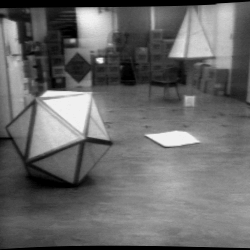
\includegraphics[width=0.6\linewidth]{img/cart_orig_left.png}
        \caption{left}
    \end{subfigure}% <- this percent sign is important 8)
    \begin{subfigure}{0.5\textwidth}
        \centering
        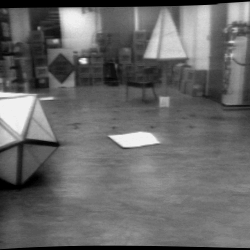
\includegraphics[width=0.6\linewidth]{img/cart_orig_right.png}
        \caption{right}
    \end{subfigure}
    \caption{An example of a stereo image.}
    \label{fig:cart_orig}
\end{figure}

The database of freely licenced stereo images we used was found at \ref{}. An example of the type of image we used is shown in figure \ref{fig:cart_orig}.

\begin{figure}
    \begin{subfigure}{0.5\textwidth}
        \begin{equation*}
            \left[
            \begin{matrix}
                7 & 7 & 5 & 4 & 0 & 0 & 0 & 0 \\
                7 & 5 & 4 & 0 & 0 & 0 & 0 & 0 \\
                6 & 5 & 0 & 0 & 0 & 0 & 0 & 0 \\
                5 & 0 & 0 & 0 & 0 & 0 & 0 & 0 \\
                5 & 0 & 0 & 0 & 0 & 0 & 0 & 0 \\
                4 & 0 & 0 & 0 & 0 & 0 & 0 & 0 \\
                0 & 0 & 0 & 0 & 0 & 0 & 0 & 0 \\
                0 & 0 & 0 & 0 & 0 & 0 & 0 & 0
            \end{matrix}
            \right]
        \end{equation*}
    \caption{left}
    \end{subfigure}%
    \begin{subfigure}{0.5\textwidth}
        \begin{equation*}
            \left[
            \begin{matrix}
                7 & 6 & 5 & 3 & 0 & 0 & 0 & 0 \\
                7 & 4 & 4 & 0 & 0 & 0 & 0 & 0 \\
                6 & 4 & 0 & 0 & 0 & 0 & 0 & 0 \\
                5 & 0 & 0 & 0 & 0 & 0 & 0 & 0 \\
                5 & 0 & 0 & 0 & 0 & 0 & 0 & 0 \\
                4 & 0 & 0 & 0 & 0 & 0 & 0 & 0 \\
                4 & 0 & 0 & 0 & 0 & 0 & 0 & 0 \\
                0 & 0 & 0 & 0 & 0 & 0 & 0 & 0
            \end{matrix}
            \right]
        \end{equation*}
    \caption{right}
    \end{subfigure}
    \caption{Greedy independent 64 bit allocation for the stereo images of figure \ref{fig:cart_orig} }
    \label{fig:cart_bit_alloc}
\end{figure}

An important question in transform coding is that of bit allocation. We wish to know how many bits, i.e. how many codevectors, to assign to each DCT coefficient to optimally recover the source. In the point-to-point case (\sysIIN, \sysJJN), this problem was studied in \ref{julien}. A simple greedy algorithm optimally allocates bits to the DCT coefficients. The algorithm assumes that the $(0,0)$ coefficient (the DC coefficient) is Gaussian, while the other 63 coefficients are Laplacian \ref{julien}. An example of how this algorithm allocates bits to the images of figure \ref{fig:cart_orig} is given in figure \ref{fig:cart_bit_alloc}.

\begin{figure}
    \begin{equation*}
        \left[
        \begin{matrix}
        0.443 & -0.01  & -0.093 & -0.011 & -0.061 &   0.003 & -0.017 &  0.062 \\
        0.416 &  0.006 & -0.011 &  0.014 & -0.031 &  -0.039 &  0.003 & -0.045 \\
        0.498 & -0.061 & -0.01  &  0.074 & -0.034 &  -0.017 &  0.008 &  0.054 \\
        0.438 &  0.027 & -0.008 &  0.074 & -0.016 &   0.022 &  0.006 & -0.004 \\
        0.449 &  0.075 & -0.019 &  0.017 &  0.014 &   0.063 & -0.029 &  0.007 \\
        0.632 &  0.028 & -0.034 & -0.018 &  0.033 &  -0.037 &  0.032 &  0.061 \\
        0.765 &  0.177 & -0.032 & -0.063 & -0.033 &   0.076 & -0.001 &  0.089 \\
        0.679 &  0.148 &  0.028 &  0.04  &  0.046 &  -0.013 &  0.046 &  0.034
        \end{matrix}
        \right]
    \end{equation*}
    \caption{DCT coefficient correlation matrix of the stereo images in figure \ref{fig:cart_orig} }
\end{figure}

\begin{figure}
    \begin{equation*}
        \left[
        \begin{matrix}
        0.654 & 0.134 & 0.054 & 0.087 & 0.077 & 0.124 & 0.119 & 0.144 \\
        0.371 & 0.072 & 0.043 & 0.059 & 0.05  & 0.063 & 0.053 & 0.048 \\
        0.273 & 0.067 & 0.065 & 0.06  & 0.055 & 0.05  & 0.062 & 0.059 \\
        0.23  & 0.056 & 0.064 & 0.053 & 0.046 & 0.045 & 0.047 & 0.039 \\
        0.242 & 0.053 & 0.05  & 0.056 & 0.047 & 0.062 & 0.058 & 0.036 \\
        0.213 & 0.064 & 0.064 & 0.05  & 0.061 & 0.052 & 0.045 & 0.059 \\
        0.238 & 0.068 & 0.07  & 0.056 & 0.048 & 0.046 & 0.042 & 0.054 \\
        0.233 & 0.081 & 0.074 & 0.066 & 0.046 & 0.05  & 0.039 & 0.049
        \end{matrix}
        \right]
    \end{equation*}
    \caption{Average DCT coefficient correlation matrix of the dataset of 39 pairs of stereo images}
\end{figure}

The DCT computations and image manipulation was coded in Python using Pillow Imaging library and numpy.

The bit allocation problem for the two source case was not studied. We have thus omitted bit allocation from our simulations.

% Implementation:
% Python PILLOW library & numpy

\subsection{Design Summary}
% Summary initialization scheme in summary. We also have two stages : training stage (which is performed offline) and running stage which is used during simulation.
To recap, and to provide an overall picture, we will now give an overview of the system design. The following describes our process for images.

\medskip
{\noindent \bf Training Phase}
\begin{enumerate}
    \item Choose pairs of stereo images to act as the training sets;
    \item Convert pixel data of stereo images to 64 scalar pair sets of 2-D DCT coefficients;
    \item Find good bit allocation using the optimal bit allocation greedy algorithm for independent sources;
    \item Uniformly quantize sets;
    \item Perform `Initialization Stage' quantization with splitting on each set;
    \item \label{channel_opt_stage}
    Perform `Channel-Optimization Stage' quantization until convergence on each set;
    \item Perform simulated annealing to find approximately optimal channel codeword mappings $b_X, b_Y$ on each set;
    \item Return to step \ref{channel_opt_stage} until satisfactory distortion is achieved.
\end{enumerate}
\medskip
{\noindent \bf Simulation Phase}
\begin{enumerate}
    \item Choose a pair of stereo images to act as the simulation set;
    \item Convert pixel data of stereo images to 64 scalar pair sets of 2-D DCT coefficients;
    \item Uniformly quantize sets;
    \item Using codebooks and channel codeword maps from training phase, find the nearest neighbour for each quantized level;
    \item Send encoded channel indices over a simulated channel;
    \item Receive indices and decode according to the centroid condition.
\end{enumerate}

% Summarize design and talk about complexity.
% [unif Q_X] -> [enc X] -> [b_X] \
%                                 --> [MAC]-- [Joint decode]
% [unif Q_Y] -> [enc Y] -> [b_Y] /
